\chapter{Models}

Typing sentences can be seen as a Markovian process. To correct sequences using HMMs, we can assume the 
hidden states to be representing the intended words, while the observations are the typed words.
We will consider two optimality criteria. The first one chooses the states that are individually most likely and 
maximizes the expected number of correct individual states. The model that implements this criterion is the 
Noisy Channel Model \ref{}.
The second criterion estimates the most likely state sequence, or \textit{trellis path}. The model and algorithm 
used to implement this criterion is the Hidden Markov Model and the \textbf{Viterbi} algorithm \ref{}.


\section{Noisy Channel Model}
The \textbf{error model} implemented in this project is called \textit{Noisy Channel Model}.
In this model we treat the original word (the misspelled word) as if a correctly spelled word had been “distorted” 
by passing through  a noisy communication channel. This channel introduces “noise” in the form of substitutions 
or other changes to the letters, making it hard to recognise the “true” word. \\


\textbf{Non-word errors} are detected by looking for any word not found in a dictionary. To correct them we first 
generate \textbf{candidates}, according to a distance given as a parameter to the model (\texttt{edit\_distance}), 
that are real words with a similar letter sequence to the error. 


This noisy channel model is, therefore, a kind of Bayesian inference.
Having an observation $x$ (a misspelled word), we want to find the word $w$ that generated this misspelled word (the intended word).
Out of all possible words in our language model $L$ we want to find the word $\hat{w}$ that maximised the 
probability $P(\hat{w}|x)$

\begin{equation}\label{eq:4.1}
\hat{w} = \arg\max_{w \in V} P(w|x) \mbox{.}
\end{equation}

Applying Bayes's rule, factoring out the denominator, since $P(x)$ doesn’t change for each word because we 
are always asking about the most likely word for the same observed error $x$,  and limiting $L$ such that we're 
going to consider only a set of candidates $C$ at a maximum edit distance for the word $x$, we get the formula:
\begin{equation}\label{eq:4.2}
\hat{w} = \arg\max_{w \in V} {P(x|w)P(w)} \mbox{.}
\end{equation}

The distance used to limit the set of candidates $C$ is the \textbf{Levenshtein} edit distance \ref{}.	

\begin{figure}[H]
	\centering
	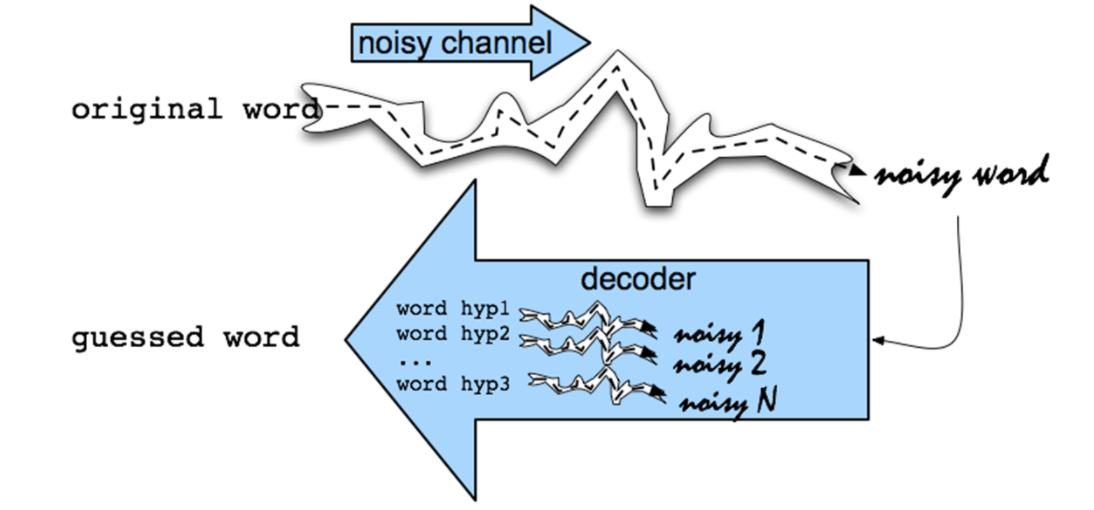
\includegraphics[width=10cm]{NoisyChannel.png}
	\caption{Diagram of the Noisy Channel Model}
	\label{fig:noisychannel}
\end{figure}

Once obtained a set of candidates, the formula \ref{eq:4.2} requires us to compute the two components, 
respectively, the prior probability of a hidden word $w$ and the channel model (or likelihood).
The prior probability $P(w)$ is given by the language model, that is obtained by counting the frequencies of 
each word in a corpus of text.  
The channel model $P(x|w)$ used in this project makes the assumption that $P(\mbox{balbo}|\mbox{bilbo}) = 
P(\mbox{a}|\mbox{i})$. The channel error model is trained on a corpus of spelling errors coming from different 
datasets. In particular, it is estimated just using the number of times that the a letter $i$ was substituted for the 
letter $a$. 

Considering each character of an alphabet $A$, generally, we'll have a confusion matrix $|A|\times|A|$ for each 
kind of channel model we're going to use. The following are the channel models used in this project:
\begin{itemize}
	\item \textsc{character deletions}: $\mbox{del}[x, y] = \frac{\mbox{count (xy  typed as x)}} 
	{\mbox{count (xy)}}$
	\item \textsc{character insertions}: $\mbox{ins}[x, y] = \frac{\mbox{count (x  typed as xy)}} 
	{\mbox{count (x)}}$
	\item \textsc{substitution of characters}: $\mbox{sub}[x, y] = \frac{\mbox{count (x  typed as y)}} 
	{\mbox{count (x)}}$
	\item \textsc{transposition of adjacent characters}: $\mbox{swap}[x, y] = \frac{\mbox{count (xy  typed as 
	yx)}} 
	{\mbox{count (xy)}}$
\end{itemize}


This model is appropriate for estimating the likelihood of \textbf{non-word spelling errors}, or errors were the 
misspelled word isn't in the vocabulary (e.g. writing \textsl{giraffe} as \textsl{graffe}).
\textbf{FIXME}: When for a input typo we do not have any candidate ?? 

\textbf{Real-word errors}, or errors were the misspelled word is in the vocabulary (e.g. writing \textsl{work}  as  
\textsl{worm}), need a slightly different approach.

We're still searching for the candidate that maximizes formula \ref{eq:4.2}, but the channel model is treated 
differently. 
We need to assume, since the word is in the vocabulary, that the input word is not actually an error. We will call 
$P(w|w)$ as $\alpha$. For this measure, we can make different assumptions about what should its value be, 
according to the writing task associated with the text. \textcolor{red}{For example, we can say that 
professionally editing a text has an alpha of $0.99$, while casually texting someone has an alpha of $0.80$.}

So, given a typed word $x$, let the channel model $P(x|w)$ be alpha when $x = w$, and then distribute 
$1-\alpha $ evenly over all other candidate corrections of $C(x)$ 

\begin{equation}\label{eq:4.3}
	P(x|w) = \begin{cases} 
	\alpha & \mbox{if } x = w \\ 
	\frac{1-\alpha}{|C(x)|} & \mbox{if }  x \in C(x) \\
	0 & \mbox{otherwise} 
	\end{cases}
\end{equation}

We'll then replace the edit probability of the various confusion matrices for non-word spelling errors with an 
equal distribution of $1-\alpha$, while keeping the logic of the model intact.

\textbf{FIXME}: When for a input typo we do not have any candidate ?? 


\section{Hidden Markov Model}

A \textbf{Hidden Markov Model} (HMM) allows us to talk about both observed events, like misspelled words that 
we see in the input, and hidden events, like the intended words, that we think of as causal factors in our 
probabilistic model. 

Our HMM is specified by the following components:
\begin{itemize}
	\item $Q = q_1q_2 \dots q_N$: a set of $N$ \textbf{states}
	\item $A=a_{11}	\dots a_{ij} \dots a_{NN}$: a \textbf{transition probability matrix} $A$. \\ Each $a_{ij}$ 
	representing the probability of moving from state $i$ to state $j$, such that $\sum_{j=1}^N a_{ij}=1 \quad 
	\forall i$. In our case, the state transitions are given by the probability of one word given its predecessor, 
	obtained by a certain corpus of text.
	\item $O = o_1o_2 \dots o_T$: a sequence of $T$ \textbf{observations}, each one drawn from a vocabulary 
	$V = v_1,v_2,\dots,v_V$
	\item $B = b_i (o_t )$: a sequence of \textbf{observation likelihoods}, also called \textbf{emission 
		probabilities}, each expressing the probability of an observation to being generated from a state $i$. These 
	are given by a corpus of misspelling errors.
	\item $\pi = \pi_1,\pi_2,\dots,\pi_N$: an \textbf{initial probability distribution} over states. $\pi_i$ is the 
	probability that the Markov chain will start in state $i$. 
\end{itemize}

\textbf{FIXME}{Aggiungere immagine fig come fig 2 di Articolo.pdf }

We consider a \textit{first-order} Hidden Markov Model, that instantiates two simplifying assumptions. First, as 
with a first-order Markov chain, the probability of a particular state depends only on the previous state. Second, 
the probability of an output observation $o_i$ depends only on the state that produced the observation $q_i$ 
and not on any other states or any other observations.

For every observed word, we will consider a subset of the every possible word as its correct candidate, given by 
the error model described in the next section.

Typing being a sequential process, as the HMM proceeds from state to state, we will also have to limit the 
candidates generated by each observation with only those having an actual transition from state $Q_{i-1}$ to 
$Q_i$.

In figure \ref{fig:trellis} we present an example of the evolution of an HMM for the sentence "\textsl{someone 
	else alwais has to cary on the storry}".

\textbf{FIXME}
\begin{figure}[H]
	\centering
	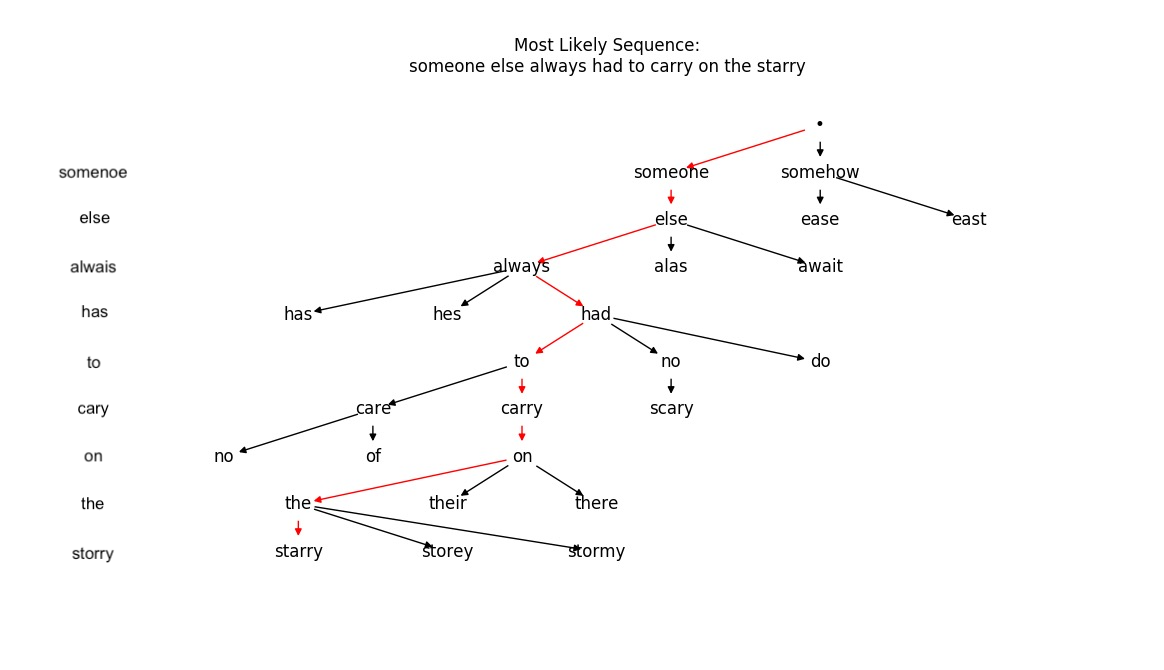
\includegraphics[width=15cm]{TrellisExample.png}
	\caption{Trellis example}
	\label{fig:trellis}
\end{figure}

In this example, the most likely state sequence \textsl{someone else always had to carry on the starry}. In this 
case, the algorithm partially fails, because the intended sentence was \textsl{someone else always has to carry 
	on the story}.


\section{Most Likely State Sequence}

The Viterbi algorithm calculates the most probable sequence of hidden states, the words intended.
The Viterbi algorithm is a probabilistic extension of minimum edit distance. Instead of computing the “minimum 
edit distance” between two strings, Viterbi computes the “maximum probability alignment” of one string with 
another. 

The initial probability of being in a state $i$, $\pi_i$, in our case the probability of intend a word $i$, and the 
transition probabilities $A_{ij}$, or the transition from the word $i$ to the next word $j$, are given. Since we have 
observed the output $y_1, y_2, \dots , y_t$, that is the sentence written with typos, it is possible to computed the most 
likely state sequence $x_1, x_2, \dots , x_t$, the sentence intended, starting from the following expression:

\begin{equation}
\begin{aligned}
V_{1,t+1} &= P(x_1, \dots, x_t, x_{t+1}, y_1, \dots, y_t,  y_{t+1}) = \\
&= \arg\max_{x_{1:t}} p(x_1, \dots, x_t | y_1, \dots, y_t) = \\
& =  \alpha \cdot p(y_{t+1}|x_{t+1})\cdot\max_{x_t} \Big( p(x_{t+1}|x_t) \max p(x_1, \dots, x_{t}|y_1, 
\dots, y_t)\Big)
\end{aligned}
\end{equation}

%FIXME
The initial state probabilities $\pi$ are actually the word frequencies (? We don’t estimate it in a proper way), the state 
transition probabilities are given by the probability of a word given its predecessor, \textbf{FIXME}: {come vengono prese} 
and the emission probabilities are the probabilities to type word $i$ when word $j$ was intended.

In our implementation, we construct the \textit{trellis} choosing the \textbf{FIXME}: {locally/globally} best state. 
\\
\textbf{FIXME}: (pi la probabilità iniziale del prima stato non lo abbiamo, non lo facciamo perchè dal nostro 
dataset non 
abbiamo sempre la prima parola…)
\textbf{NOTA}: in Articolo.pdf del progetto non parla mai di probabilita' iniziale ma considera sempre solo il 
language model, a sto punto possiamo mettere la nota sopra tra i possibili miglioramenti nelle conclusioni

We decide to implement the \textbf{Viterbi} based algorithm instead the Forward-Backward algorithm relying on 
the 
experiments carried out in the literature.
The HMM-Based Error Correction Mechanism for Five-Key Chording Keyboards article \cite{tarniceriu2015hmm} 
explains 
that the Forward-Backward algorithm estimates the most likely state for each observation, but the resulting state 
sequence may not be a valid succession of words in natural language (or a very unlikely word sequence) and 
produce 
inferior results.


